\textbf{Problem statement: }Write a pass that instruments an input benchmark to count the number of times each instruction executes
\textbf{Problem instance: }
\begin{itemize}
\item count program instructions at runtime
\item output-per instruction count
\end{itemize}

\subsection{Pass description}
The pass differs from the prior pass in that it instruments the target byte code to perform an analysis on itself. After instrumentation, the benchmark program executes and dynamically counts instructions, outputting the total at termination. This dynamic analysis is therefore two phase with phase 1 being the opt pass and phase 2 being program execution.\\
First we describe the intended instrumented binary diagrammatically in Figure\ref{Part2transform}\\

\begin{figure}[here]
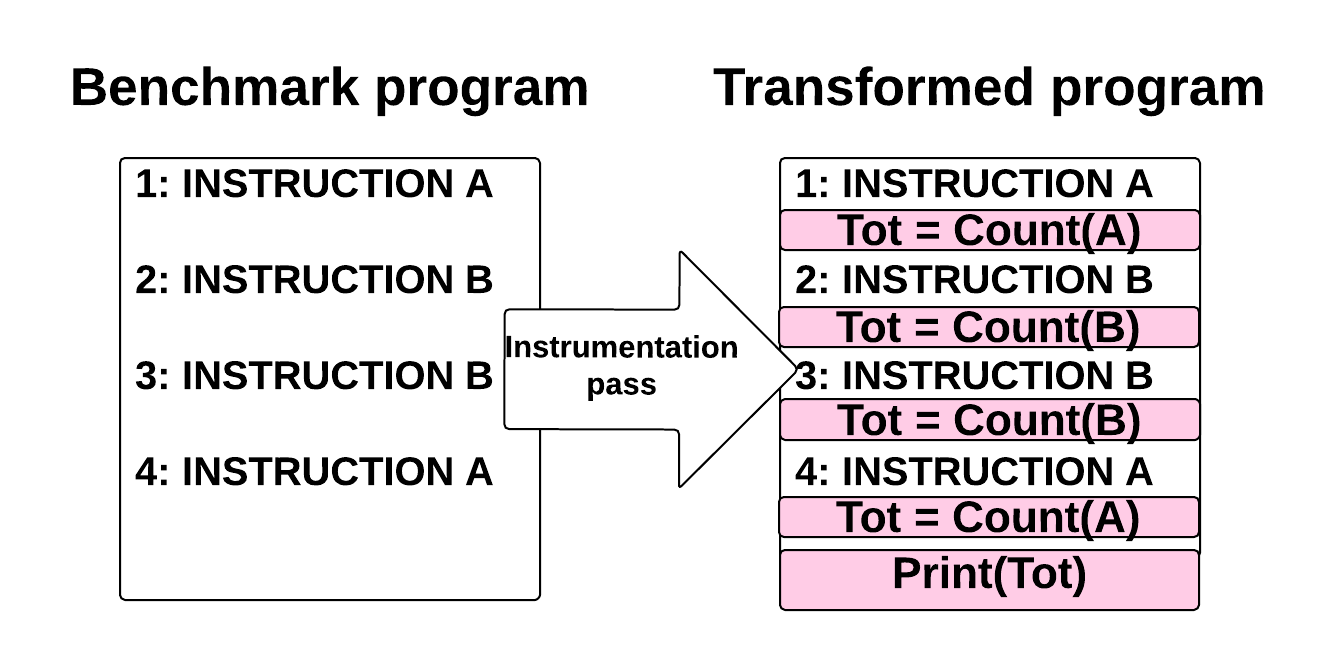
\includegraphics[width=0.4\textwidth]{CompilersProj1Part2Diag.png}
\caption{Required bytecode transformation}
\label{Part2transform}
\end{figure}

With a target binary defined we describe a code transformation that the opt pass must perform:
\begin{algorithm}
 \KwIn{$I$}
 $x \gets 0$\\
 $i \gets$ ref($I$.at(0)) \\
 \While{$i + 1 \neq 0$}
 { 
 	
 	$i' \gets$ \textbf{Count}(valAt($i$))\\ 
 	$i$.insertBefore($i'$)\\
 	$i$ += 1\\
 }
 $i \gets$ ref($I$.last())\\
 $i$.insertBefore(\textbf{print}())

 \caption{Dynamic instruction count instrumentation pass}
\end{algorithm}
where:\\
$I$ is an input program instruction list in LLVM byte code (.bc) format\\
$i$ is an individual instruction iterator $I$\\

The \textit{count()} function can be recycled from section the \textit{static count} pass. Similarly the \textit{Print()} function can be recycled.

\subsection{Instrumentation pass implementation summary}
Besides the skills used for the static pass, implementation of the dynamic pass presented challenges of inserting instrumentation functions to the test bench code and further augmenting that code to call inserted functions.\\
Ensuring instrumentation functions were in scope during the opt pass was documented in the one of the project breif "hints" sections. Counting sorted lists of instructions was a probem solved during the static instruction count problem. Therefore the major challenges were: 
\begin{itemize}
\item Finding a function signature in LLVM byte code
\item Inserting a call to a function signature above a byte code instruction
\item Passing parameters to an inserted function call
\end{itemize}

Finding a function signature \textbf{COSTAS IMPROVED THIS, I WILL SAY NO MORE}\\

Inserting a function call 
